\documentclass[t,12pt,numbers,fleqn,usenames,xcolor=dvipsnames]{beamer}

%\documentclass[t,12pt,numbers,fleqn,handout]{beamer}
% The theme: https://github.com/kailashbuki/beamerthemesaarland`

%\usetheme[
%background=saarland,
%logo=uds
%]{saarland}
%\graphicspath{{images/}}


\usepackage{amsmath}
\usepackage{mathtools}
\usepackage{amsfonts}
\usepackage{paralist}
\usepackage{latexsym}
\usepackage{amssymb}
\usepackage{stmaryrd}
\usepackage{phonetic}
\usepackage{wasysym}
\usepackage{pgf}
\usepackage{tikz}
\usepackage{url}
\usetikzlibrary{arrows}
\usepackage{array}
\usepackage{pgfpages} 
\usepackage{multirow} 
\usepackage{graphicx}
\usepackage{color}
\usepackage{listings,lstautogobble}
\lstset{
	basicstyle=\ttfamily,
	mathescape
}
\lstdefinelanguage{Isar}%
{morekeywords={
		_first,theory,end,types,datatype,consts,defs,primrec,
		syntax,translations,apply, lemma,theorem,corollary,
		done,sorry,goal,proof,fixed variables,_last,definition,locale},
	sensitive=true,
	morecomment=[l]{-- },
	literate=
	{\\<not>}{{$¬$}}1 {\\<times>}{{$×$}}1                 
	{\\<Rightarrow>}{{$\Rightarrow$}}1%
	{\\<equiv>}{{$\equiv$}}1 {~=}{{$\not=$}}1                         
	{\\<rightleftharpoons>}
	{{$\rightleftharpoons$}}1
	{\\<exists>}{{$\exists$}}1 
	{\\<parallel>}{{$\parallel$}}1 
	{\\<Longrightarrow>}
	{{$\Longrightarrow$}}1
	{\\<lbrakk>}{{$\lsemantics$}}1
	{\\<rbrakk>}{{$\rsemantics$}}1
	{\\<longrightarrow>}
	{{$\longrightarrow$}}1
	{\\<and>}{{$\land$}}1
	{\\<or>}{{$\lor$}}1
	{\\<bigwedge>}{{$\bigwedge$}}1
	{\\<lbrakk>}{{$\llbracket$}}1
	{\\<rbrakk>}{{$\rrbracket$}}1
	{\\<subseteq>}{{$\subseteq$}}1
	{\\<one>}{{$1$}}1	
	{\\<in>}{{$\in$}}1
	{\\<times>}{{$\times$}}1
	{\\<lparr>}{{$\llparenthesis$}}1
	{\\<rparr>}{{$\rrparenthesis$}}1
	{\\<lambda>}{{$\lambda$}}1
	{\\<^bsub>}{{$_$}}0
	{\\<^esub>}{{$_$}}0
	{\\<>}{{$\llparenthesis$}}1
	{\\<otimes>}{{$\otimes$}}1
	{ü}{"u}1 {ä}{"a}1 {ö}{"o}1 
	{Ü}{"U}1 {Ä}{"A}1 {Ö}{"O}1 {ß}{{ss}}1
}[keywords,comments,strings]%
\usepackage{hyperref}
\usepackage{verbatim}
\usepackage{fancyvrb}
\usepackage{tabularx}
\usepackage{tikz}
\usepackage{tikz-cd}
\usetikzlibrary{cd}
\usepackage{graphicx}
\usepackage{collectbox}
\usepackage{tabularx}
\usepackage{wrapfig}
\usepackage{lscape}
\usepackage{textcomp}

\usepackage[show]{ed}
\usepackage{smartdiagram}
\usesmartdiagramlibrary{additions}
\usepackage{adjustbox}
\setlength{\arrayrulewidth}{1mm}
\setlength{\tabcolsep}{18pt}
\renewcommand{\arraystretch}{1.5}
\hypersetup{colorlinks=false,
    linkcolor=blue,
    citecolor=blue,
    filecolor=blue,
    urlcolor=blue,
    unicode=false}

%\usepackage{macros}
%\usepackage{local}
%\usepackage{basics}

% To include lagda 

\usepackage{adjustbox}

%\usepackage{agda-stdlib/latex/agda}

\usepackage{amssymb}
\usepackage{bbm}
\usepackage[greek,english]{babel}
\usepackage{ucs}
\usepackage[utf8]{inputenc}
\usepackage{autofe}
\DeclareUnicodeCharacter{8988}{\ensuremath{\ulcorner}}
\DeclareUnicodeCharacter{8989}{\ensuremath{\urcorner}}
\DeclareUnicodeCharacter{8803}{\ensuremath{\overline{\equiv}}}


\usepackage{catchfilebetweentags}
%\usepackage{fancyvrb}
%\DefineVerbatimEnvironment
%{code}{Verbatim}

\usepackage{prooftree1} 
\usepackage{macros}

\lstset{language=lisp,basicstyle=\ttfamily,breaklines=true,showspaces=false,showstringspaces=false,breakatwhitespace=true,texcl=true,escapeinside={\%*}{*)}}
\tikzstyle{stuff_fill}=[rectangle,draw,fill=black!20,minimum size=1.4em]


\usepackage{fancybox}

\mode<presentation>{}


\usetheme{default}
\setbeamertemplate{navigation symbols}{} 
\setbeamertemplate{itemize item}[ball]
\setbeamersize{text margin left = 4mm}
\setbeamersize{text margin right = 4mm}

%\input{def-beamer}

\title{Leveraging Information in Theory Presentations}
\author{Yasmine Sharoda\\ \vspace{0.5cm} Supervisors: Jacques Carette and William Farmer}
\institute[]{Department of Computing and Software, McMaster University}
\date{July 8,2019}
	
\newcommand\textline[4][t]{%
	\par\smallskip\noindent\parbox[#1]{.333\textwidth}{\raggedright\texttt{+}#2}%
	\parbox[#1]{.333\textwidth}{\centering#3}%
	\parbox[#1]{.333\textwidth}{\raggedleft\texttt{#4}}\par\smallskip%
}	
\newcommand{\hilight}[1]{\colorbox{yellow}{#1}}
\setbeamertemplate{footline}{%
	\raisebox{5pt}{\makebox[\paperwidth]{\hfill\makebox[10pt]{\scriptsize\insertframenumber}}}}

%\newcommand{\hilight}[1]{\colorbox{yellow}{#1}}	
	
\begin{document}

\begin{frame}
\titlepage
\end{frame}

\begin{comment}
\vfill
%\begin{center}
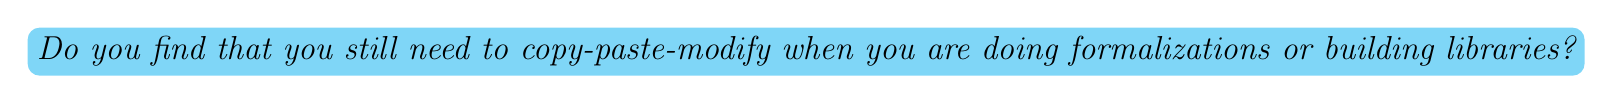
\begin{tikzpicture}
\node[preaction={fill=cyan,fill opacity=0.5},rounded corners=1ex,font=\fontsize{12pt}{12pt}\itshape] 
{Do you find that you still need to 
copy-paste-modify 
when you are doing formalizations or building libraries?};
\end{tikzpicture}
%\end{center}
\vfill
\end{comment}

\section{Motivation}
\begin{comment}[fragile]
\begin{tikzpicture}[overlay, remember picture]
\node[anchor=center] at (current page.center) {
	\begin{beamercolorbox}[center]{title}
Do you find yourself going through \\
\textbf{copy-paste-modify} flow?
	\end{beamercolorbox}};
\end{tikzpicture}
\end{comment}

\subsection{Agda Example}
\begin{frame}[fragile]
\frametitle{Defining Homomorphism}
\begin{columns}
	\begin{column}{0.45\textwidth}
\scriptsize		
		\lstset{emph={} ,emphstyle=\fbox}
		\begin{lstlisting}[mathescape]
theory Foo { 
  U : type 
  s1 : U 
  s2 : U $\to$ U $\to$ U
}
		\end{lstlisting}
\pause		
		\begin{lstlisting}
theory FooHom{
  f1 , f2 : Foo 
  h : f1.U $\rightarrow$ f2.U 
  pres-s1 : h f1.s1 = f2.s1  
  pres-s2 : h (f1.s2 x y) 
            = f2.s2 (h x) (h y)
}
		\end{lstlisting}
	\end{column}
	\begin{column}{0.45\textwidth}
\pause		
\scriptsize
	 	\begin{lstlisting}
theory Bar {
  U : type 
  s1 : U 
  s2 : U $\rightarrow$ U 
}
	 	\end{lstlisting}
\pause
		\begin{lstlisting}
theory BarHom { 
  b1, b2 : Bar 
  h : b1.U $\rightarrow$ b2.U 
  pres-s1 : h s1 = s2  
  pres-s2 : h (b1.s2 x) 
            = b2.s2 (h x)
}
		\end{lstlisting}
	\end{column}
\end{columns}
\end{frame}

\begin{frame}[fragile]
\frametitle{Defining Homomorphism}
\begin{columns}
\scriptsize
\begin{column}{0.45\textwidth}
		\lstset{emph={generates Hom} ,emphstyle=\fbox}	
	\begin{lstlisting}
theory Foo { 
  U : type 
  s1 : U 
  s2 : U $\to$ U $\to$ U
} $\hilight{generates Hom}$
	\end{lstlisting}
\end{column}
\begin{column}{0.45\textwidth}
	\begin{lstlisting}
theory Bar {
  U : type 
  s1 : U 
  s2 : U $\rightarrow$ U 
} $\hilight{generates Hom}$
	\end{lstlisting}
\end{column}
\end{columns}
\end{frame}
%\frametitle{Example: Agda\footnote{code from: 
%\url{https://github.com/JacquesCarette/TheoriesAndDataStructures/}}}
%Define the category of group
%\begin{lstlisting}

%\end{lstlisting}
%\begin{columns}
%	\begin{column}{0.45\textwidth}
		
%		Agda monoid, TwoSorted, Pointed, AbelianGroup
%source: 
%https://github.com/JacquesCarette/TheoriesAndDataStructures/blob/master/Structures/TwoSorted.lagda
% \\
%source: 
%https://github.com/JacquesCarette/TheoriesAndDataStructures/blob/master/Structures/Pointed.lagda
% \\
%source: 
%https://github.com/JacquesCarette/TheoriesAndDataStructures/blob/master/Structures/AbelianGroup.lagda
%	\end{column}
%	\begin{column}{0.45\textwidth}
%       Agda Involutive
       %\footnote{source: 
       %\url{https://github.com/JacquesCarette/TheoriesAndDataStructures/blob/master/Structures/InvolutiveAlgebra.lagda}}
       %		
%	\end{column}
%\end{columns}


\begin{comment}[fragile]
\frametitle{Real Example: Agda Library}
\ExecuteMetaData[agdacode/Morphism.tex]{groupHom}
\end{comment}



\begin{frame}
\frametitle{Real Example: Agda Library
\footnote{\tiny{ source: 
\url{https://github.com/agda/agda-stdlib/blob/master/src/Algebra/Morphism.agda}}}}
\begin{onlyenv}<1>
	\begin{tabular}{l}	
		\includegraphics[scale=0.25]{agda_example/hom_def_hr.png}\\		
		\includegraphics[scale=0.25]{agda_example/mon_morph_hr.png}\\
		\includegraphics[scale=0.25]{agda_example/cmon_morph_hr.png}\\		
	\end{tabular}	
\end{onlyenv}
\begin{onlyenv}<2>
	\begin{tabular}{l}	
		\includegraphics[scale=0.25]{agda_example/hom_def_hr.png}\\		
		\includegraphics[scale=0.25]{agda_example/group_morph_hr.png}	
	\end{tabular}	
\end{onlyenv}		
\end{frame}

\subsection{Real Example: Isabelle Library}
\begin{comment}[fragile]
\frametitle{Example: Isabelle 
\footnote{\tiny{source: \url{https://isabelle.in.tum.de/dist/library/HOL/HOL-Algebra/index.html}}}}
\begin{columns}
	\begin{column}{0.45\textwidth}
		\begin{figure}
			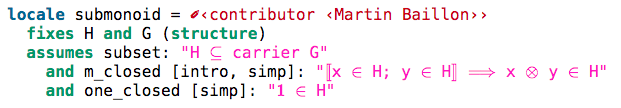
\includegraphics[scale=0.3]{isabelle_example/submonoid.png}
		\end{figure}
		\begin{figure}
			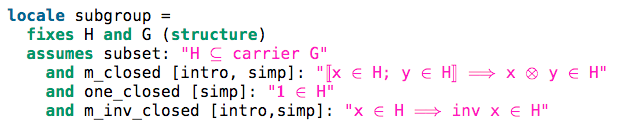
\includegraphics[scale=0.3]{isabelle_example/subgroup.png}
		\end{figure}
	\end{column}
	\begin{column}{0.45\textwidth}
		\begin{figure}
			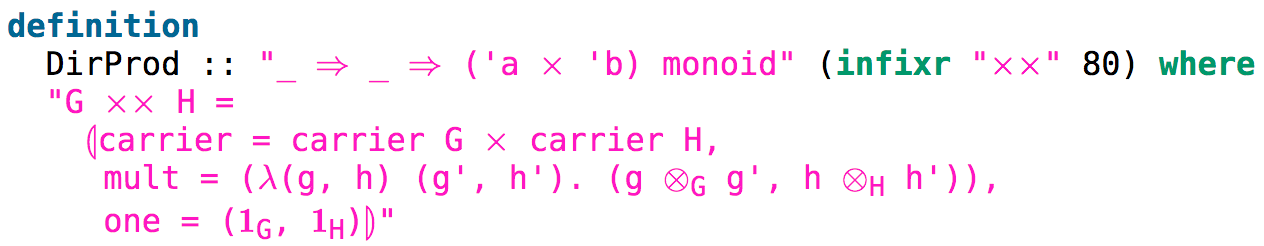
\includegraphics[scale=0.2]{isabelle_example/prod_hr.png}
		\end{figure}
		\begin{figure}
			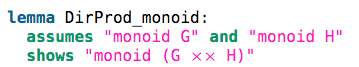
\includegraphics[scale=0.3]{isabelle_example/prod_mon.png}
		\end{figure}
		\begin{figure}
			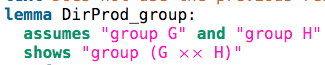
\includegraphics[scale=0.3]{isabelle_example/prod_group.png}
		\end{figure}
	\end{column}
\end{columns}
\end{comment}

\begin{frame}[fragile]
\frametitle{Example: Isabelle \footnote{\tiny{source: 
			\url{https://isabelle.in.tum.de/dist/library/HOL/HOL-Algebra/index.html}}}}
\begin{onlyenv}<1>
\begin{tabular}{l}	
	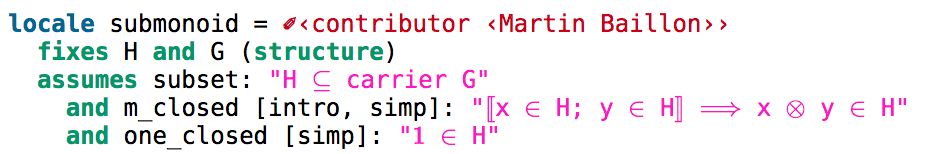
\includegraphics[scale=0.3]{isabelle_example/submon_hr.png}\\		
	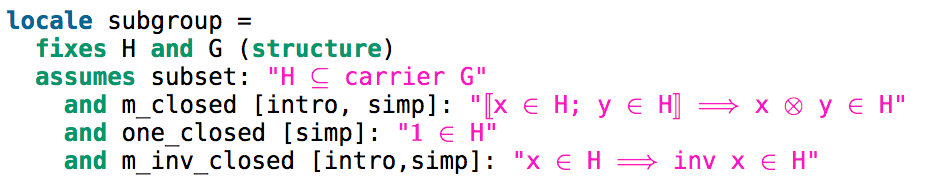
\includegraphics[scale=0.3]{isabelle_example/subgroup_hr.png}
\end{tabular}	
\end{onlyenv}		
\begin{onlyenv}<2>
\begin{tabular}{l}	
	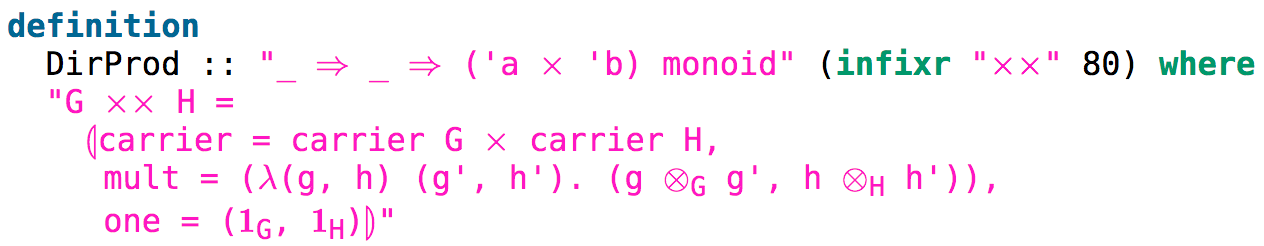
\includegraphics[scale=0.2]{isabelle_example/prod_hr.png}\\		
	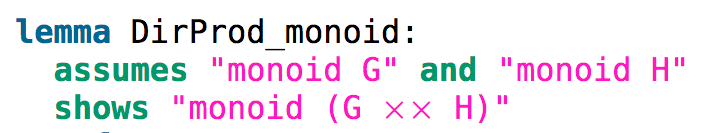
\includegraphics[scale=0.2]{isabelle_example/prod_mon_hr.png}\\
	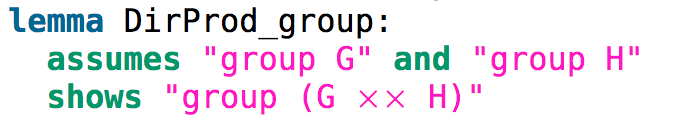
\includegraphics[scale=0.2]{isabelle_example/prod_group_hr.png}
\end{tabular}	
\end{onlyenv}		

\end{frame}

\begin{comment}
\frametitle{Example: Isabelle \footnote{\tiny{source: 
\url{https://isabelle.in.tum.de/dist/library/HOL/HOL-Algebra/index.html}}}}
\scriptsize
\begin{lstlisting}
DirProd :: "_ $\Rightarrow$ _ $\Rightarrow$ ('a $\times$ 'b) monoid" (infixr "$\times \times$" 80) 
where "G $\times \times$ H =
$\llparenthesis$ carrier = carrier G $\times$ carrier H,
mult = ($\lambda$(g, h) (g', h'). (g $\otimes\textsubscript{G}$ g', h $\otimes\textsubscript{H}$ h')),
one = (1$\textsubscript{G}$, 1$\textsubscript{H}$ $\rrparenthesis$"
\end{lstlisting}
\lstinputlisting[language=Isar, firstline=711, lastline=713]{isabelle_example/Group.thy}
\lstinputlisting[language=Isar, firstline=723, lastline=725]{isabelle_example/Group.thy}
\end{comment}

\subsection{Other Structures}
\begin{frame}
\frametitle{Other Structures?}
\vspace{0.15cm}
{\scriptsize
	Signature, Sub-algebra, Product-algebra, Projection of product algebra, Congruence-relation on 
	an algebra, Quotient algebra, Record definition of a theory, Homomorphism, 
	Homomorphism-equality, Composition of morphisms, Kernel of Homomorphism, Isomorphism, 
	Endomorphism, Automorphism, Closed term language, Open term language, Staged terms, 
	Structural induction, Evaluation function for terms, Simplification of terms, Rewrite rules, 
	Sub-terms of a term language, Equivalence of terms, Parse trees, Homomorphism between 
	terms and trees. 
}

\vspace{0.3cm}
\pause
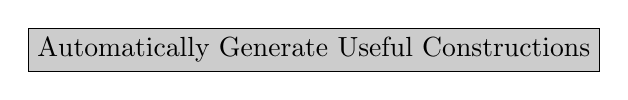
\begin{tikzpicture}
\draw (1, 1) node [stuff_fill] {Automatically Generate Useful Constructions};
\end{tikzpicture}
\
\end{frame}

\begin{frame}
\frametitle{Why is that Useful?}
\begin{itemize}
\item Avoid Boilerplate 
\begin{itemize}
	\item Distracts user from original task 
	\item Error-prone and not reusable 
	\item Does not communicate information about the structure 
\end{itemize}
\item Reduce the amount of labor associated with building rich libraries 
\end{itemize}
\end{frame}

\begin{comment}[fragile]
	\begin{center}
	\smartdiagramset{
		uniform color list=white!60!black for 3 items, 
		back arrow disabled=true, 
		text width=2cm,
		additions={
			additional item offset=0.85cm,
			additional item border color=red,
		}
	}
	\smartdiagramadd[flow diagram:horizontal]{%
		Abstract, Compute, Generate %
	}{%
		below of module1/Abstraction, below of module3/Specialization
	}
	\end{center}
\end{comment}

\section{Algebraic Theories}
\begin{frame}[fragile]
\frametitle{Algebraic Theories}
\begin{itemize}
\item well-typed dependent record. It contains	
	   \begin{itemize}
	   	\item sorts
	   	\item typed symbols
	   	\item axioms 
	   \end{itemize}
\begin{figure}[ht]
	\begin{proofrules}
		\[ \ \justifies \varnothing \ \wfctx \]
		\[ \Gamma\ \wfctx \qquad x\notin |\Gamma| 
		\qquad \Gamma \vdash \sigma : \kappa : \Box \justifies
		(\Gamma\ ;\ x : \sigma)\ \wfctx \]
	\end{proofrules}
%	\caption{Formation rules for contexts}
	\label{fig:ctx}
\end{figure}   
   \pause
   \item How are they presented in formal systems?
\end{itemize}
\end{frame}
\begin{comment}
Third formation rule 
\end{comment}

\begin{frame}[fragile]
\frametitle{Monoid Theory}
\only<1>{
	\begin{figure}
		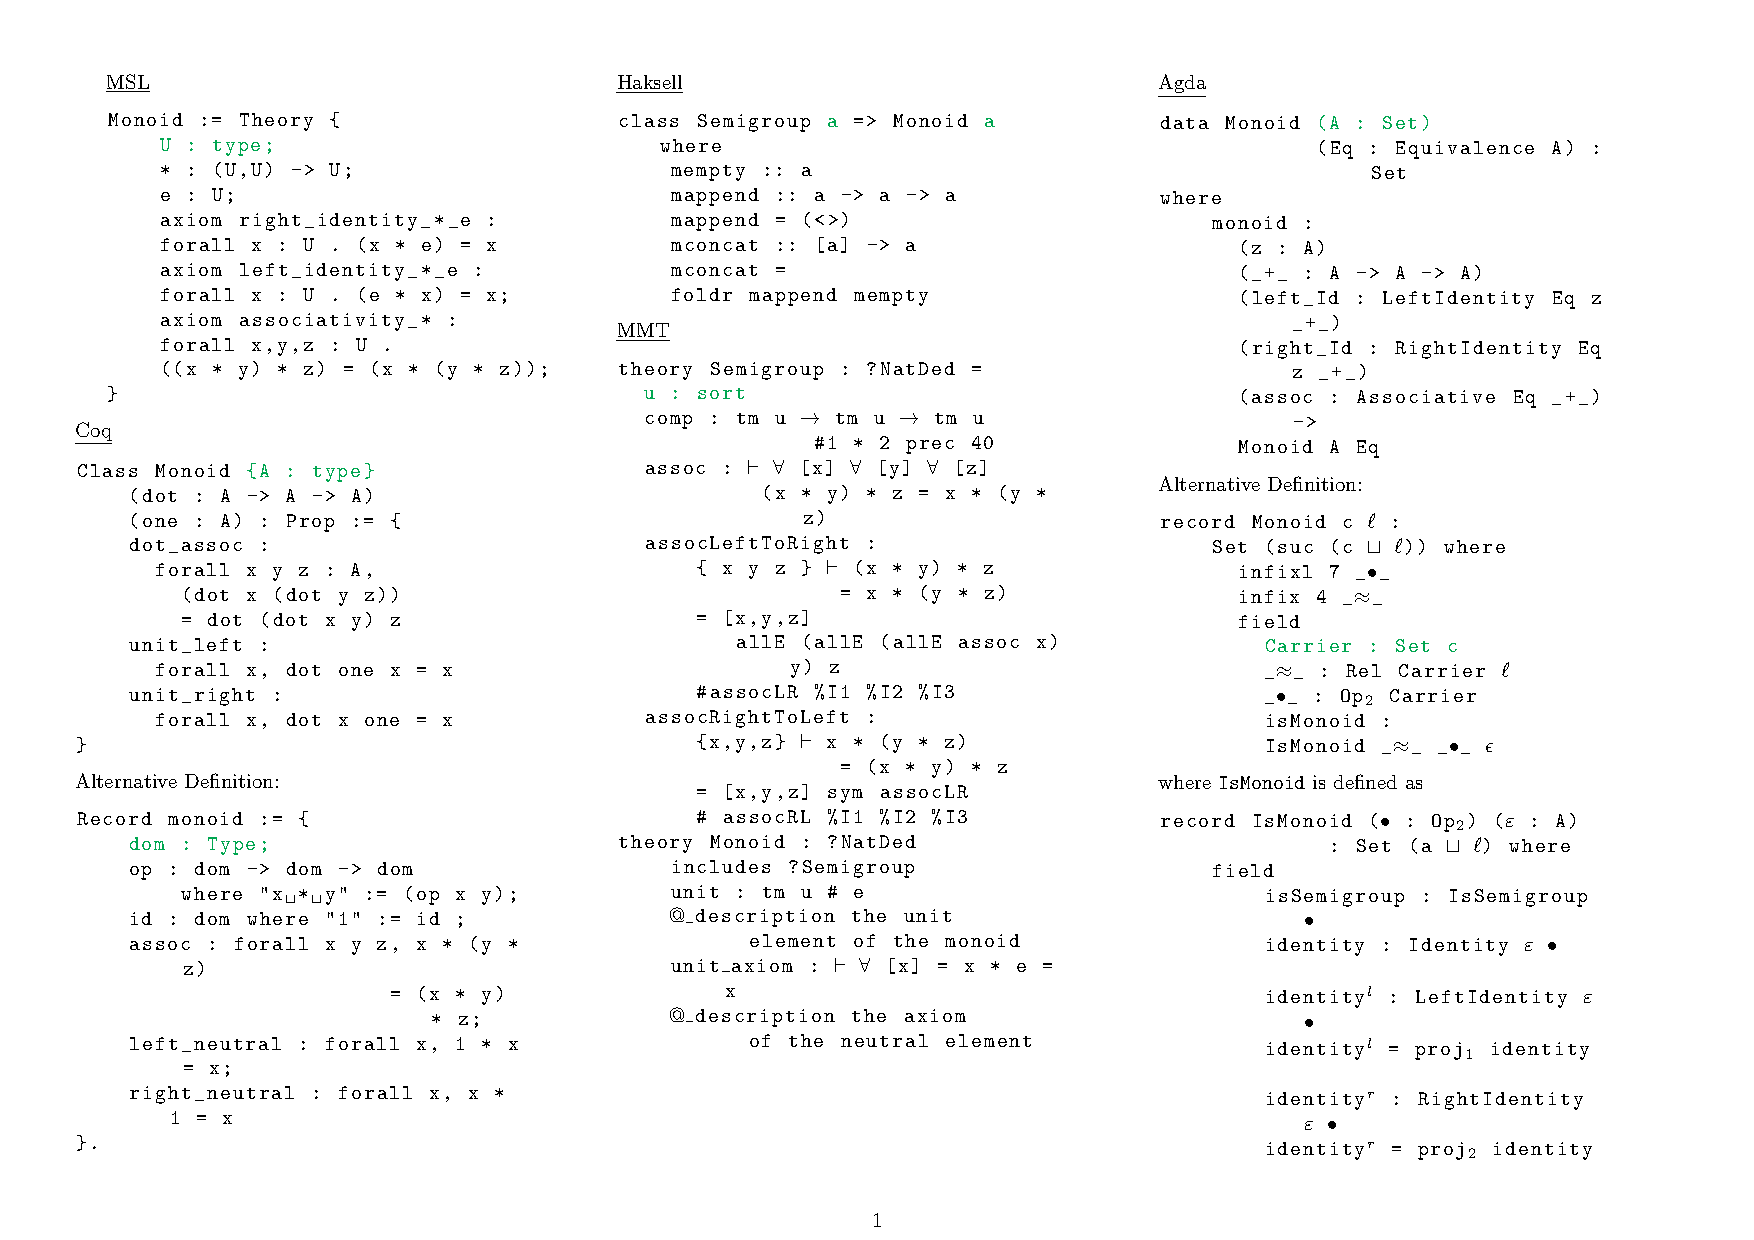
\includegraphics[scale=0.4]{monoid_highlighted.pdf}
	\end{figure}
}
\only<2>{
	\begin{tikzpicture}
	\draw (0, 0) node[inner sep=0] {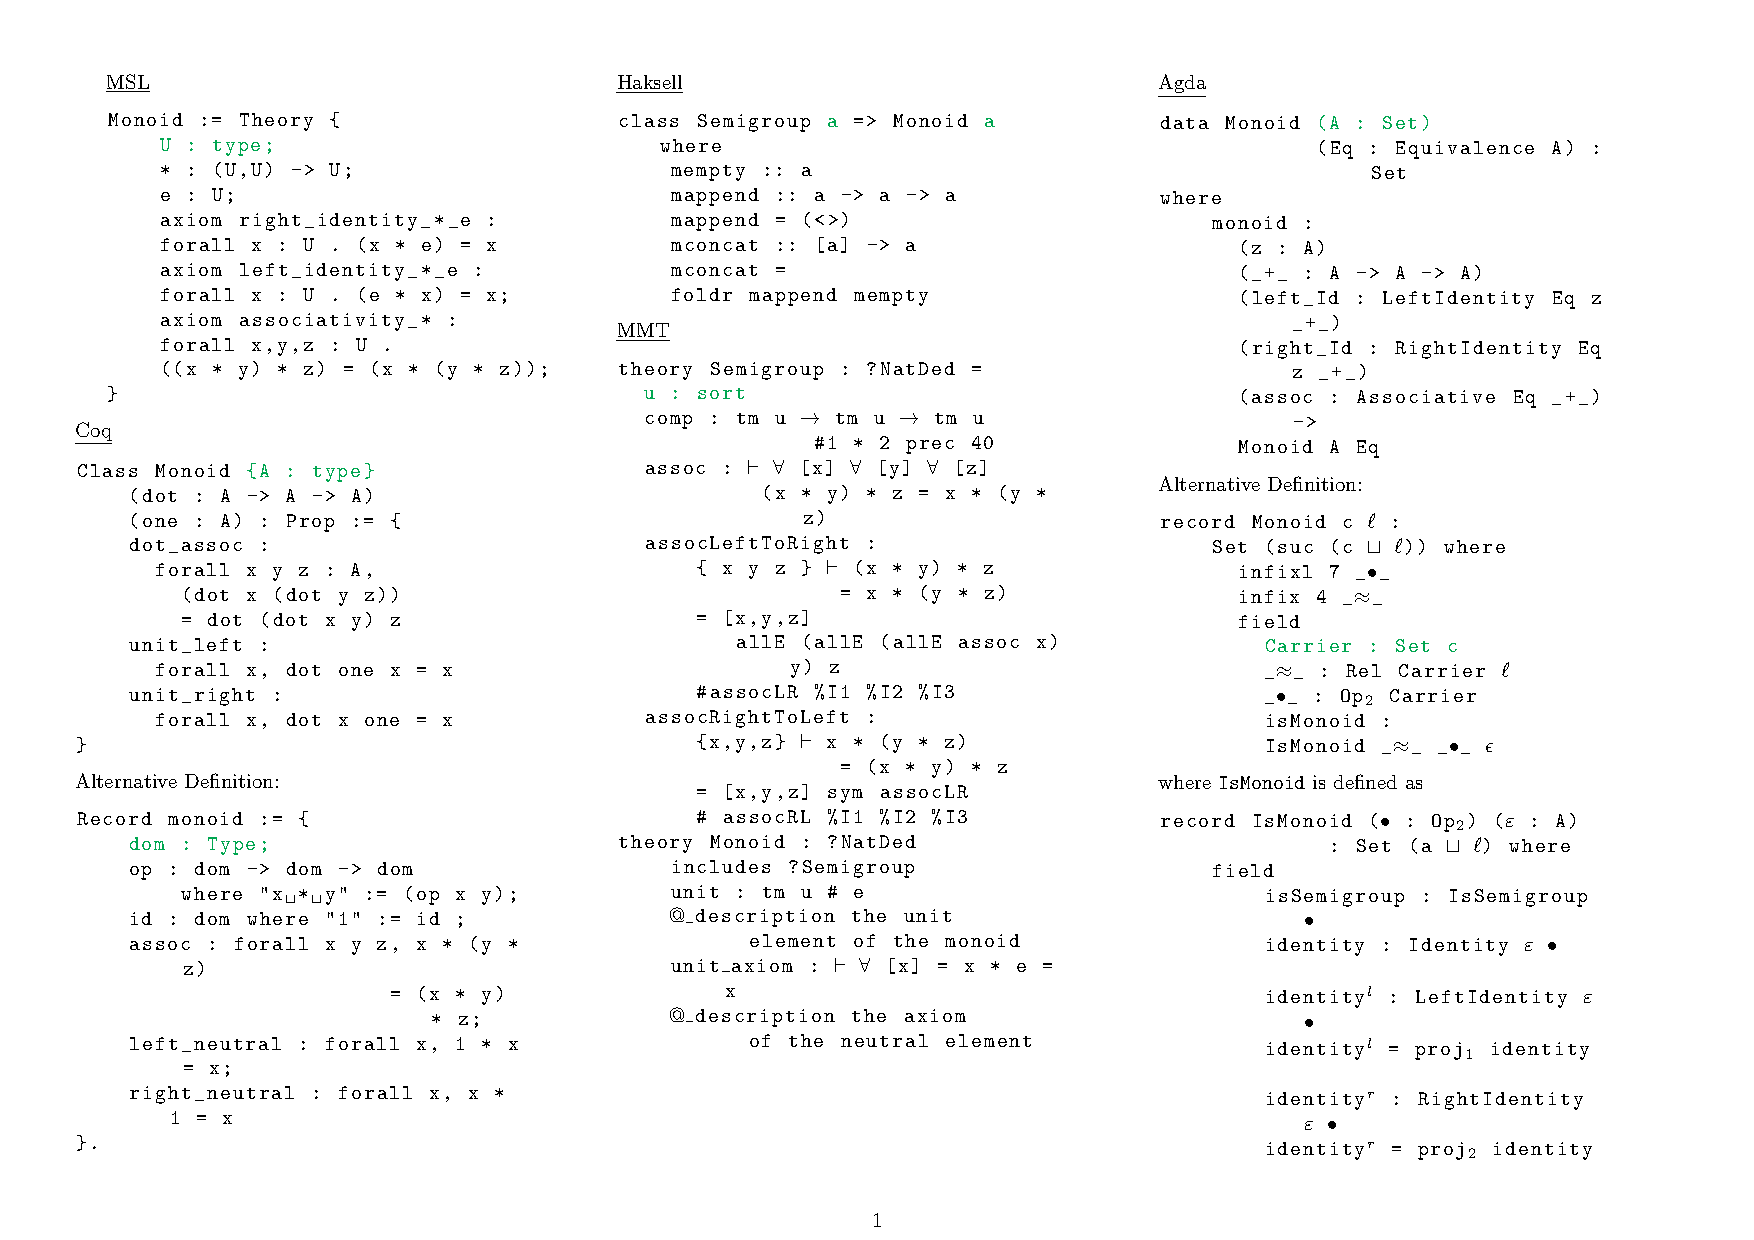
\includegraphics[scale=0.38]{monoid_highlighted.pdf}};
	\draw (0.5, 1) node [stuff_fill] {Abstract Over Details of Theory Presentations};
	\end{tikzpicture}
}
\end{frame}

\section{Research Objectives}
\begin{frame}
\frametitle{Research Objectives}
\begin{itemize}
	\item \textcolor{blue}{Abstracting} over representation language 
	\begin{itemize}
		\item Generate Useful Algebraic Structures 
	\end{itemize}
	\item \textcolor{blue}{Specializing} to different languages
	  \begin{itemize}
	  	\item Different Syntax
	  	\item Different Foundation 
	  	\item Example: Isabelle/HOL and Agda 
	  \end{itemize}
\end{itemize}
\end{frame}

\section{Approach}
\begin{frame}[fragile]
\frametitle{Abstraction: Use MMT}
We use MMT as a framework to abstract over syntax of theory presentations 
\begin{itemize}
	\item Platform Independent 
	\item Simple Module System
	\item Example: 
\scriptsize	
	\begin{lstlisting}
theory Magma : FOL = 
  U : type
  op : U $\to$ U $\to$ U # 1 $\circ$ 2
theoy AdditiveMagma : FOL = 
  U : type
  + : U $\to$ U $\to$ U 
view additive : Magma $\to$ AdditiveMagma = 
   U := U 
   op := +   
	\end{lstlisting}
\end{itemize}
\end{frame}

\begin{comment}[fragile]{Generating Structures}
Manipulating OmDoc terms 
\end{comment}

\begin{frame}[fragile]{Translating Definitions: Domain Analysis}
\begin{itemize}
	\item Domain Scoping 
\scriptsize{	
	\begin{tabular}{ p{1cm} p{1cm} p{1cm} p{1cm}}
		MathScheme & MMT & Agda & Lean \\ [1ex]
		Coq & Haskell &  Isabelle & Idris 
	\end{tabular}}
\normalsize
	\item Data Collection 
	\begin{itemize}
		\item Foundations 
		\item Module System 
		\item Supported Features 
	\end{itemize}
	\item Data Analysis 
	\begin{itemize}
		\item Commonlities, Differences and Dependencies 
	\end{itemize}
\end{itemize}
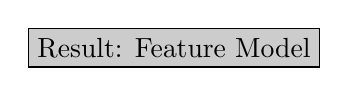
\begin{tikzpicture}
\draw (0,0) node [stuff_fill] {Result: Feature Model};
\end{tikzpicture}
\end{frame}

\begin{frame}[fragile]{Feature Model}
Consists of 
\begin{itemize}
	\item Feature Diagram: Hierarchies and Dependencies
	\begin{itemize}
		\item Mandatory, Alternative or Optional 
	\end{itemize}
	\item Feature Definition
	\item Composition Rules
	\begin{itemize}
		\item Valid/Invalid Feature Combinations 
	\end{itemize}
	\item Rationale
	\begin{itemize}
		\item Reasons for choosing / not choosing a feature
	\end{itemize} 
\end{itemize}
\end{frame}

\section{Evaluation}
\begin{frame}[fragile]
\frametitle{Evaluation: MathScheme Library}
\scriptsize	
\begin{lstlisting}
theory Carrier := Empty extended_by {U : type}
theory Magma := Carrier extended_by {_$\circ$_ : U $\to$ U $\to$ U}
theory Pointed := Carrier extended_by {e : U}
theory AddtivieMagma := Magma rename {$\circ$ := +}
\end{lstlisting}
\vfill
\begin{tikzcd}
	Carrier \arrow[r,hook] \arrow[d,hook] & Pointed  & \\
	Magma \arrow[d,mapsto] & &  \\
	AdditiveMagma &  &  \\
\end{tikzcd}	
\end{frame}

\begin{frame}[fragile]
\frametitle{Evaluation: MathScheme Library}
\scriptsize	
\begin{lstlisting}
theory Carrier := Empty extended_by {U : type}
theory Magma := Carrier extended_by {_$\circ$_ : U $\to$ U $\to$ U}
theory Pointed := Carrier extended_by {e : U}
theory AddtivieMagma := Magma rename {$\circ$ := +}
theory PointedMagma := Combine Pointed {} Magma {}
\end{lstlisting}
\vfill
\begin{tikzcd}
	Carrier \arrow[r,hook] \arrow[d,hook] \arrow[rd,hook]& Pointed \arrow[d,hook] & \\
	Magma \arrow[d,mapsto] \arrow[r,hook] & PointedMagma & \\
	AdditiveMagma & & \\
\end{tikzcd}	
\end{frame}

\begin{frame}[fragile]
\frametitle{Evaluation: MathScheme Library}
\scriptsize	
\begin{lstlisting}
theory Carrier := Empty extended_by {U : type}
theory Magma := Carrier extended_by {_$\circ$_ : U $\to$ U $\to$ U}
theory Pointed := Carrier extended_by {e : U}
theory PointedMagma := Combine Pointed {} Magma {}
theory AddtivieMagma := Magma rename {$\circ$ := +}
LeftUnital := PointedMagma extended_by {left_unital : ... }
view Flip : Magma -> Magma := 
  U = U 
  * = [a , b : U] b * a 
RightUnital := Mixin LeftUnital {} Flip {}     
\end{lstlisting}
\begin{tikzcd}
	Carrier \arrow[r,hook] \arrow[d,hook] \arrow[rd,hook]& Pointed \arrow[d,hook] & \\
	Magma \arrow[d,mapsto] \arrow[r,hook] & PointedMagma \arrow[d,hook] \arrow[dr,hook]& \\
	AdditiveMagma & LeftUnital \arrow{r}{\text{Flip}} & RightUnital \\
\end{tikzcd}	
\end{frame}

\section{Conclusion}
\begin{frame}[fragile]
\frametitle{Conclusion}
\begin{itemize}
	\item A declarative language to build highly structured libraries with less human effort 
	\item A toolbox for making formalization tasks much easier 
\end{itemize}
\end{frame}

\end{document}



